\section{Experimentação Contínua}
\label{sec:ref-experimentacao-continua}

Na literatura, a Experimentação Contínua (ou \textit{Continuous Experimentation}, \textit{CE}) recebe diferentes denominações, como desenvolvimento orientado a dados (\textit{Data-Driven Development}), sistema de inovação experimental, entre outras \cite{erthal_characterization_2023}. Esses termos normalmente se referem ao mesmo conceito: a definição sistemática de hipóteses, entrega contínua e monitoramento de métricas para avaliação de ideias com base em evidências do uso do \textit{software} em seu contexto real \cite{fagerholm_right_2017}.

Essa prática surgiu no contexto fortemente influenciado pela metodologia \textit{Lean} e tem se tornado cada vez mais comum no mercado, sendo adotada por grandes organizações como Facebook, Google e Microsoft \cite{issa_mattos_hurrier_2023}. Diversos benefícios já foram apresentados na literatura, como aumentar a probabilidade de atender às expectativas dos usuários e aumentar seu engajamento, prevenindo o abandono do serviço, o que pode impactar significativamente a receita anual de um produto \cite{erthal_characterization_2023}.

Apesar de todos os seus benefícios, implementar um sistema de experimentação contínua pode ser desafiador, dado que, além dos testes A/B, esse processo envolve diversas outras atividades e técnicas que conectam os níveis estratégico e de desenvolvimento \cite{issa_mattos_hurrier_2023}. \citeonline{erthal_characterization_2023} apresenta uma revisão da literatura visando caracterizar essas atividades, visto que não há um consenso sobre elas e, normalmente, cada companhia as executa de forma particular. Os autores reuniram e combinaram os diferentes modelos e processos encontrados na literatura e criaram um diagrama que visa descrever as principais atividades a serem realizadas em um sistema de experimentação contínua. Este modelo é apresentado na Figura \ref{fig:erthal-process}.

\begin{figure}
\centering
\caption{\textit{A Combined Process for Continuous Experimentation}}
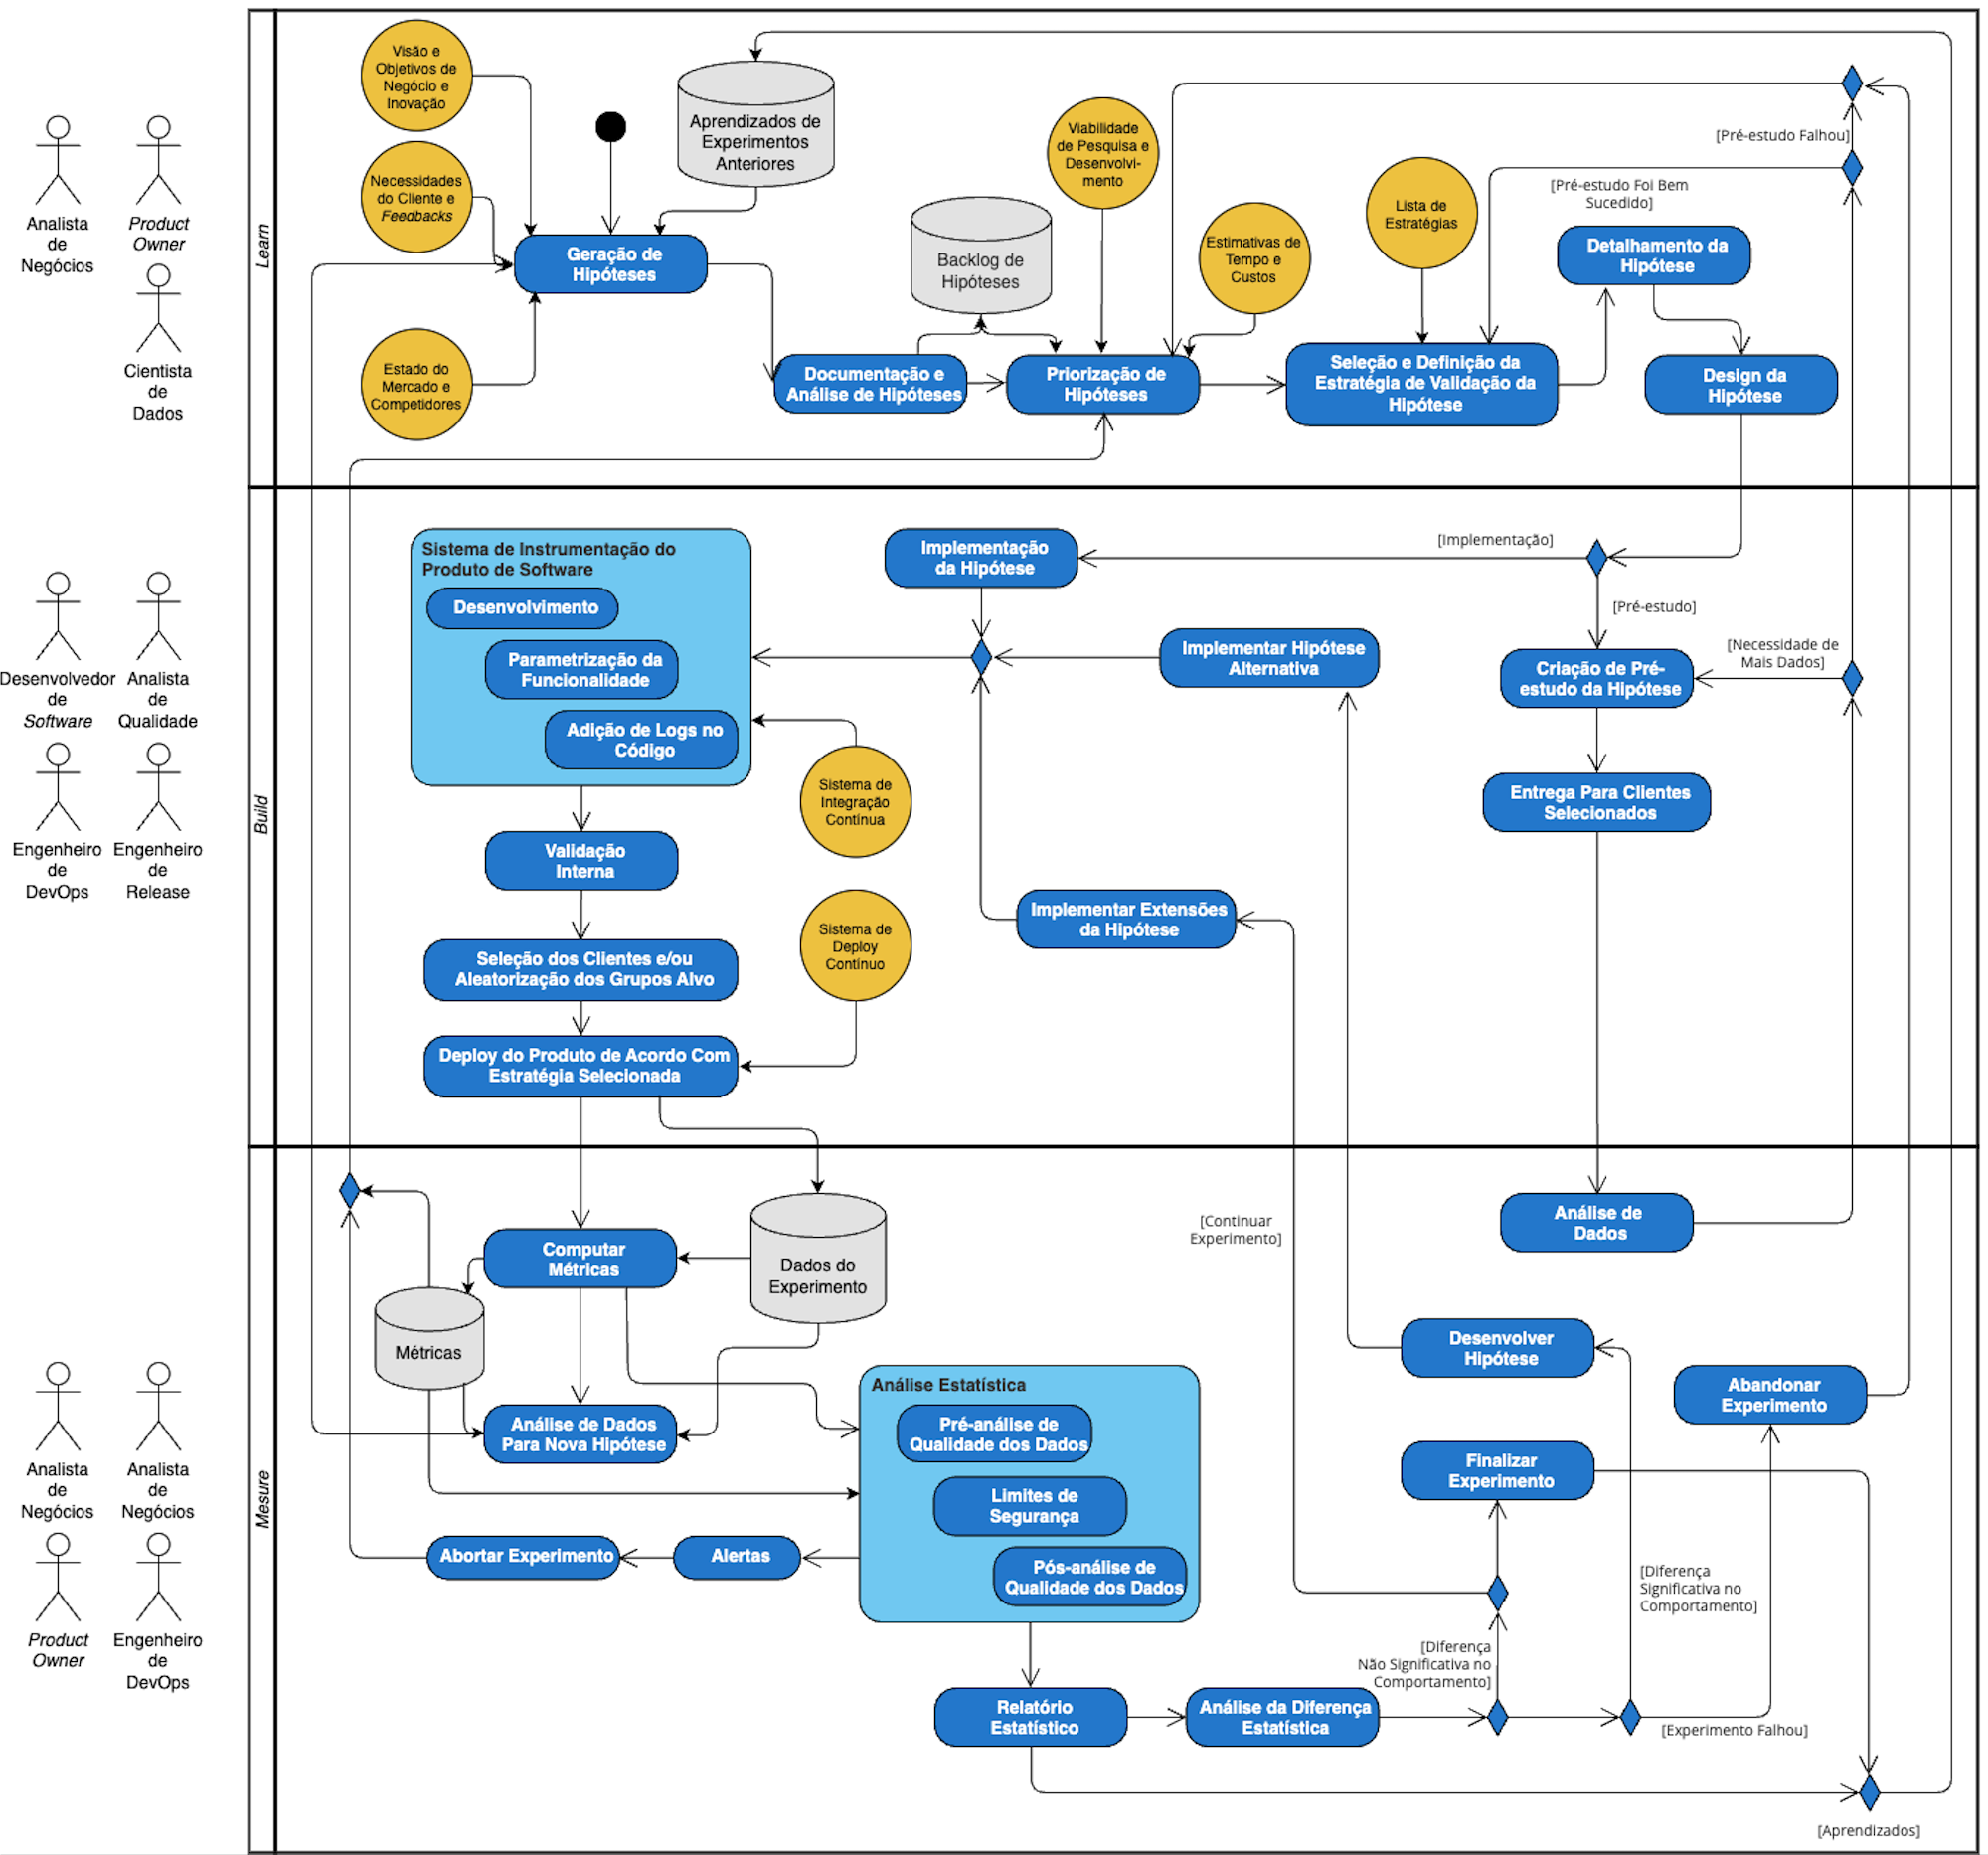
\includegraphics[width=1\linewidth]{figuras/combined_ce_process.png}
\text{Fonte: Adaptado de \citeonline{erthal_characterization_2023}}
\label{fig:erthal-process}
\end{figure}

% O artigo \citeonline{erthal_characterization_2023} realiza um trabalho minucioso na caracterização da literatura, trazendo diversos estudos primários e modelos já existentes. Por isso, o processo proposto pelos autores se apresenta como uma fonte confiável de referência. Desta forma, optou-se por guiar as atividades a serem realizadas no Estudo de Caso desta monografia a partir do modelo apresentado, analisando o processo de desenvolvimento atual do produto analisado e identificando atividades faltantes ou melhorias para as já existentes.
